% $Header: /cvsroot/latex-beamer/latex-beamer/examples/beamerexample3.tex,v 1.8 2004/10/07 20:53:07 tantau Exp $

\documentclass{beamer}

% \usepackage{bbding}
%\usepackage[utf8]{inputenc}
\usepackage[latin1]{inputenc}
\usepackage{graphicx}
\usepackage{epsfig}
%\usepackage{colortbl}
\usepackage{amsfonts}
\usepackage{verbatim}
\font\sevenex=cmex7
\scriptfont3=\sevenex \scriptscriptfont3=\sevenex
% \logo{\includegraphics[width=1.58cm]{../../../figures/code_devel/lbnl_logo.eps}}
% \useoutertheme{infolines}
% \setbeamertemplate{footline}{\raisebox{-2ex}{\pgfuseimage{institut-logo}}
%   \usebeamerfont{date in head/foot}\insertshortdate{}\hfill
%   \usebeamertemplate{navigation symbols}\hfill
%   \insertframenumber{}/\inserttotalframenumber}



\mode<presentation>
{
%    \usetheme{PaloAlto}
   \usetheme{Warsaw}

   \setbeamercovered{transparent}
} 	

% \setbeamercovered{transparent}

\title[New Generation Models]{New generation of LLRF and beam-based feedback stability models}

\author[ATG/UCB]{D. Driver, A. Queiruga, Q. Llimona, C. Serrano}

\institute[LBNL]{LBNL/UC Berkeley/UPF Barcelona}
\date[LBNL]{LBNL, Berkeley, Sept 3, 2013}



%-----------document--------------

\begin{document}

\frame{\titlepage}

\part{Index}

\frame{
  \frametitle[]{Disclaimers}
    \begin{block}{This is not a Physics talk}
      \begin{center}
	Focus on the implementation side of the modeling tools.
      \end{center}
    \end{block}
    \begin{block}{Small project}
      \begin{center}
	3 man-months total. 2 UCB PhD students 50\% time for 3 months.
      \end{center}
     \end{block}
}


\frame{

  \frametitle{Index}
%   \nameslide{Index}
%   \tableofcontents[hideallsubsections,part=1]
  \tableofcontents[hideallsubsections,part=2]
}

\defbeamertemplate*{footline}{shadow theme}
{%
  \leavevmode%
  \hbox{\begin{beamercolorbox}[wd=.5\paperwidth,ht=2.5ex,dp=1.125ex,leftskip=.3cm plus1fil,rightskip=.3cm]{author in head/foot}%
    \usebeamerfont{author in head/foot}\insertframenumber\,/\,\inserttotalframenumber\hfill\insertshortauthor
  \end{beamercolorbox}%
  \begin{beamercolorbox}[wd=.5\paperwidth,ht=2.5ex,dp=1.125ex,leftskip=.3cm,rightskip=.3cm plus1fil]{title in head/foot}%
    \usebeamerfont{title in head/foot}\insertshorttitle%
  \end{beamercolorbox}}%
  \vskip0pt%
}

\part{Contents}

\section[Context]{Context}

\frame{
	\frametitle[]{Context}
	\tableofcontents[currentsection, hideothersubsections]
}

\subsection{Motivation}

\frame{
	\frametitle[]{Motivation (1/2)}
	\begin{figure}
	  \centering
	  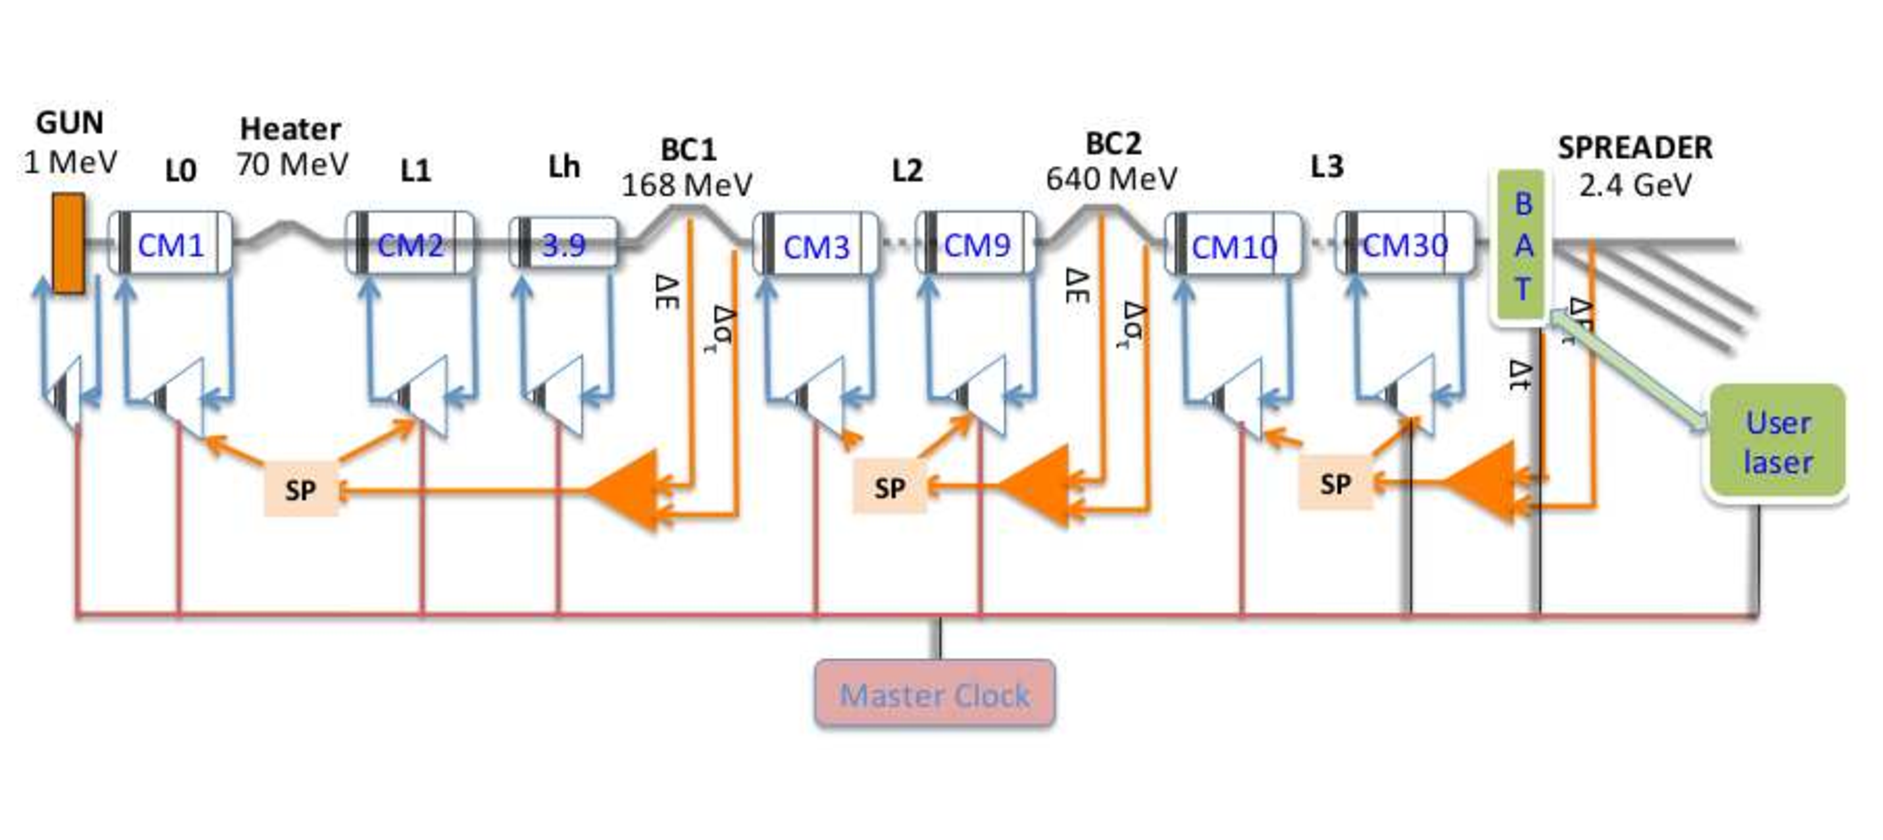
\includegraphics[scale=0.35]{figures/ngls_feedback.pdf}
	\end{figure}
}

\frame{
	\frametitle[]{Motivation (2/2)}
	\begin{figure}
	  \centering
	  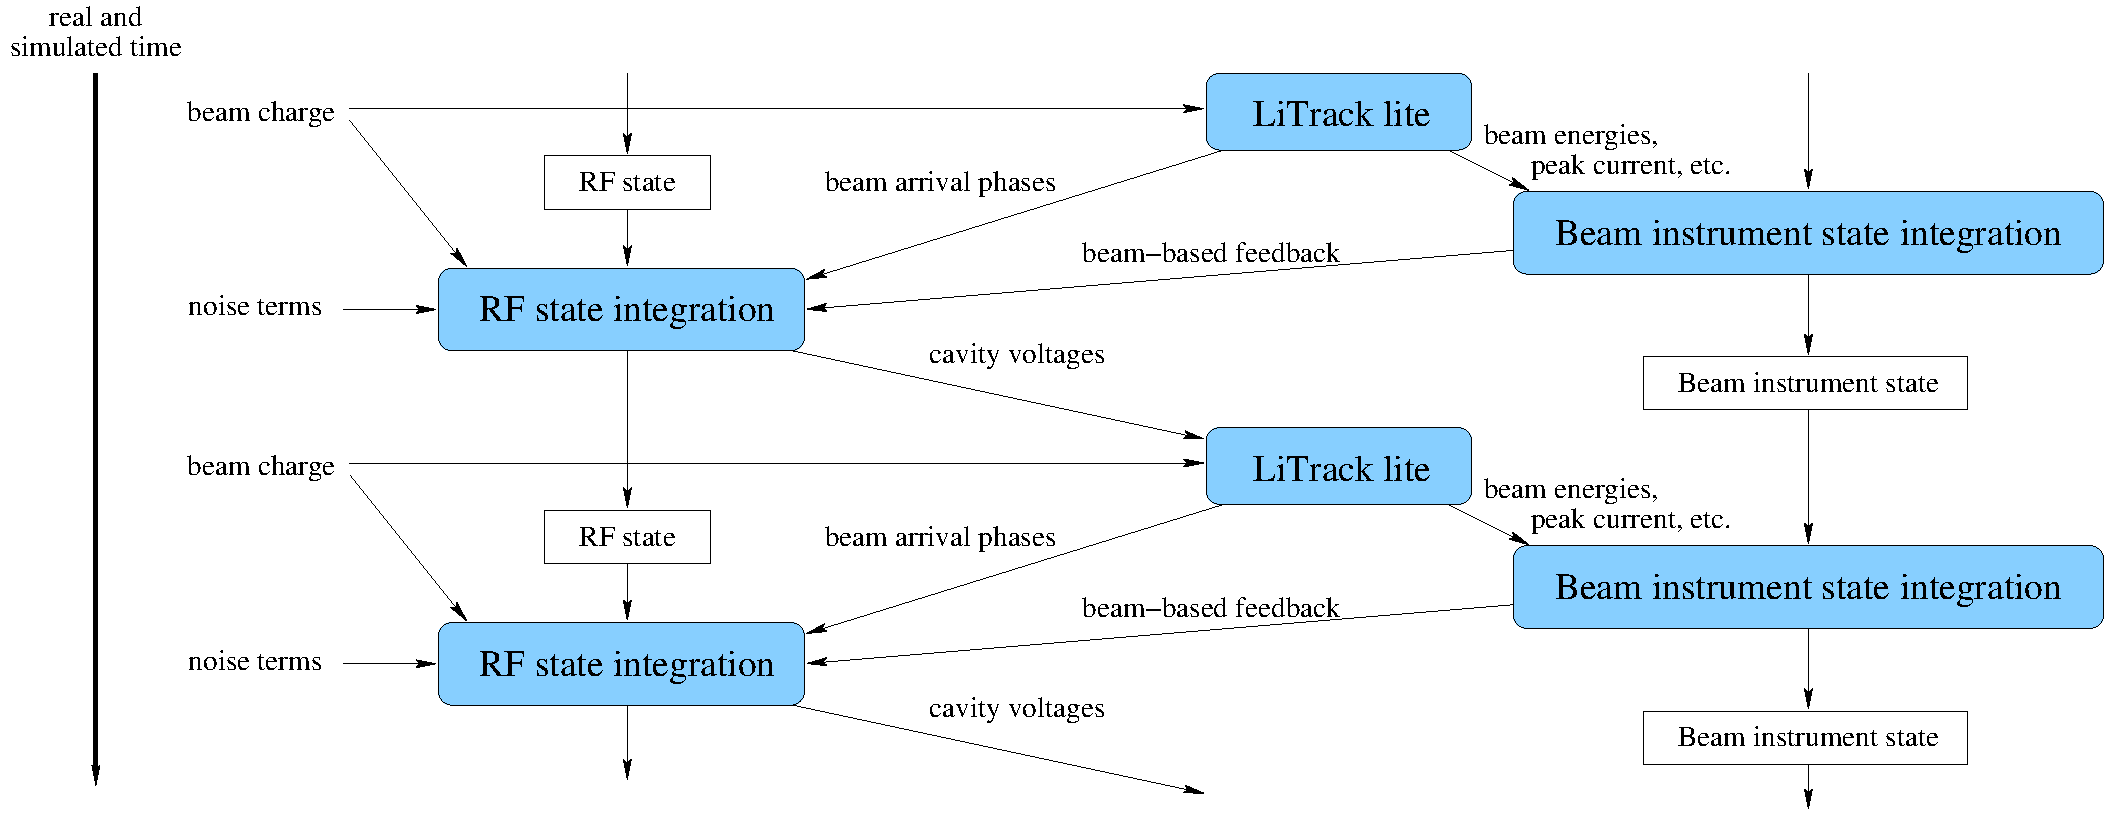
\includegraphics[scale=0.30]{figures/model_do2.pdf}
	\end{figure}
}

\subsection{NGLS Modeling effort}
\frame{
	\frametitle[]{NGLS Modeling effort}
	\begin{block}{Departing point}
		\begin{center}
		LBNL experience in LLRF and beam dynamics modeling  (separately).
		\end{center}
	\end{block}
	\begin{block}{Progressive convergence plan}
		\begin{center}
		Start in Matlab/Octave to exercise the physics, then migrate to something more computationally efficient.
		\end{center}
	\end{block}
	\begin{block}{Current status}
		\begin{center}
		We got some answers from the Physics standpoint and just migrated to a C/Python-based solution. 
		\end{center}
	\end{block}
}

\frame{
	\frametitle[]{Re-engineering Motivation}
	\begin{block}{Efficiency}
		\begin{center}
		Both from a computationally and from an operational standpoint.
		\end{center}
	\end{block}
	\begin{block}{Rigor}
		\begin{center}
		Reviewing process performed while migrating models into C/Python.
		\end{center}
	\end{block}
	\begin{block}{Flexibility}
		\begin{center}
		Generic models where configuration and interaction with high-level applications is greatly simplified. 
		\end{center}
	\end{block}
}

\subsection{LBNL/UC Berkeley Collaboration}
\frame{
  \frametitle[]{LBNL/UC Berkeley Collaboration}
    \begin{block}{ATG's Nature}
	\begin{center}
	  Dynamic, creative and curious group with didactic profiles. Plenty of interesting projects to share.
	\end{center}
    \end{block}
    \begin{block}{Overlapping fields}
	\begin{center}
	  Room for collaboration offering the opportunity for a two-way exchange.
	\end{center}
    \end{block}
    \begin{block}{Two excellent institutions: One shuttle stop a way}
      \begin{center}
	Geographical and institutional proximity, coupled with the excellence of UCB makes collaboration very attractive to LBNL for continued programs.
      \end{center}
    \end{block}

}

\section[Software Architecture]{Software Architecture}

\frame{
	\frametitle[]{Software Architecture}
	\tableofcontents[currentsection, hideothersubsections]
}

\subsection{Requirements}
\frame{
  \frametitle[]{Requirements}
    \begin{itemize}
      \item Semantically equivalent to the existing Matlab/Octave code.
      \item Performance improvements:
      \begin{itemize}
       \item Computation speed,
       \item Memory usage.
      \end{itemize}
    \item Modularity:
      \begin{itemize}
       \item Unit tests,
       \item Ease of re-implementation of different building blocks,
      \end{itemize}
      \item Configuration:
      \begin{itemize}
       \item Configuration file management: Storage and tracking,
       \item Flexibility to implement different Linac configurations easily.
      \end{itemize}
      \item High-level software interface:
      \begin{itemize}
       \item Provide API/hooks for upper level software to configure and run the models using a user-friendly interface.
      \end{itemize}

    \end{itemize}

}

\subsection{Proposed architecture}
\frame{
  \frametitle[]{Proposed architecture}
    \begin{columns}[t]
    \begin{column}[T]{0.6\textwidth}
      \begin{enumerate}
        \item User edits files in browser front-end
        \item Client sends JSON files to Server
        \item Server executes simulation Python
        \item Python configures and calls wrapped C code
        \item Output files post-processed in Python
        \item Server sends data and plots to client
        \item Browser software renders plots
        \end{enumerate}
    \end{column}
    \begin{column}[T]{0.4\hsize}
      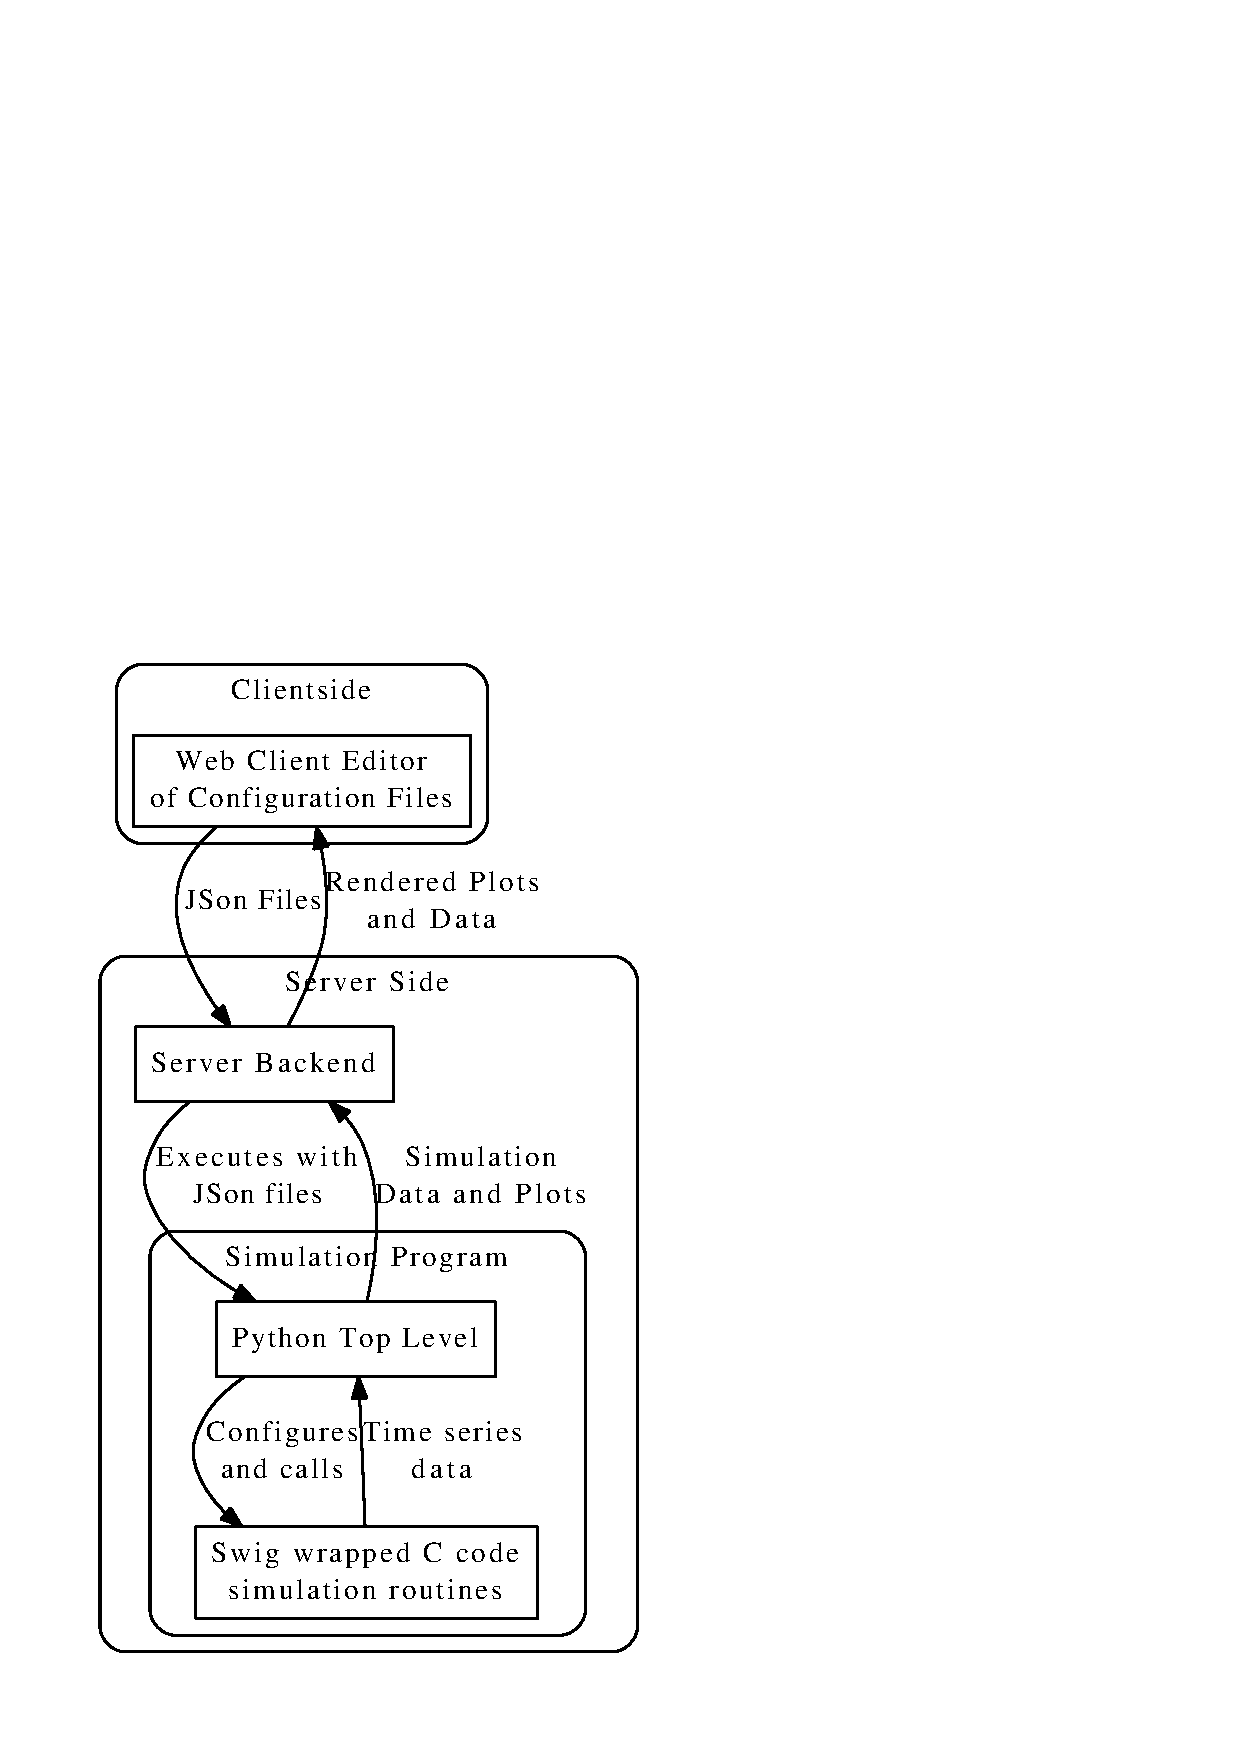
\includegraphics[height=0.9\textheight]{figures/architecture}
    \end{column}
  \end{columns}
}

\section{Implementation}

\frame{
	\frametitle[]{Implementation}
	\tableofcontents[currentsection, hideothersubsections]
}

\subsection{Simulation code structure}
\frame{
  \frametitle[]{Simulation Code Structure}
  \begin{columns}[t]
    \begin{column}[T]{0.45\textwidth}
      Simulation split into C and Python:
      \begin{itemize}
      \item Python top level for reading configuration files and post-processing.
      \item C code implementing computationally intensive inner loop.
      \item Swig automatically wraps C functions and data structures.
        \begin{itemize}
        \item Accessing C arrays from Python slightly clumsy.
        \end{itemize}
      \end{itemize}
    \end{column}
    \begin{column}[T]{0.55\hsize}
      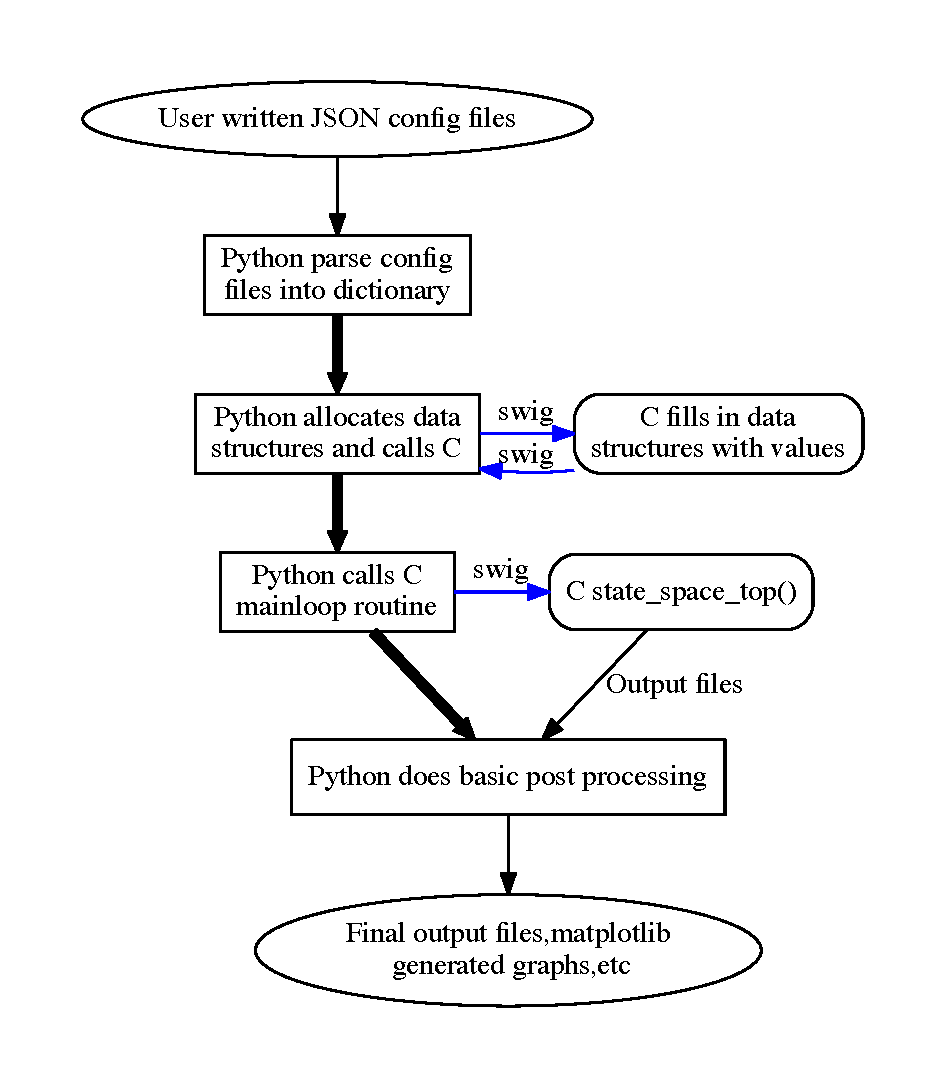
\includegraphics[height=0.9\textheight]{figures/shallowoutline}
    \end{column}
  \end{columns}
}

\subsection{Low-level code}

\frame{
  \frametitle[]{Key Internal Data Structures}
  \begin{itemize}
  \item Reusable filter data structure Filter, Filter\_State
  \item Data structures for parameters:
    \begin{itemize}
    \item LLRF: Linac\_Param, FPGA\_Param, Cavity
    \item Electron gun parameters: Gun\_Param
    \item Noise sources: Dynamic\_Param
    \item Beam-Based-Feedback: BBF\_Param
    \end{itemize}
  \item Data structures for states:
    \begin{itemize}
      \item Linac\_State, FPGA\_State, Cavity\_State
      \item Doublecompress\_State
      \end{itemize}
  \end{itemize}
}

\frame{
  \frametitle[]{Unit Tests}
  \begin{itemize}
  \item Wrote tests to validate individual pieces of code.
  \item Larger LLRF routines tested against data files generated from Octave Code.
  \item Doublecompress and BBF routines tested by calling Octave code using oct2py with random inputs.
  \item All tests can be run with one script to verify patches.
  \end{itemize}
}

\frame{
  \frametitle[]{Improvements over Octave Code}
  \begin{itemize}
  \item Speed: 1.6 hours for 6,000 steps vs. 30 seconds for 1.2 million steps. $\approx$40,000x Faster
  \item Memory: No longer storing timeseries data in memory.
  \item Flexibility: Linac structure can be rearranged and reconfigured easily in configurations.
  \item Documented and commented code.
  \item Verification via unit tests.
  \item Python top level improves development and interfacing with other codes.
  \end{itemize}
}


\subsection{Simulation Engine}

\frame{
  \frametitle[]{Simulation Engine}
  \begin{columns}[t]
    \begin{column}{0.5\textwidth}
      Work Flow in Python:
      \begin{itemize}
       \item All functions accessible
	\item Only 4 libraries
	\begin{itemize}
	\item Numpy
	\item Scipy
	\item Matplotlib
	\item JSON
	\end{itemize}
	\item One stop environment
      \end{itemize}
	Python:
	\begin{itemize}
	\item Well documented
	\item Huge user community
	\item Easy to learn
	\item Active development
	\end{itemize}
    \end{column}
    \begin{column}{0.5\hsize}

	\centering
      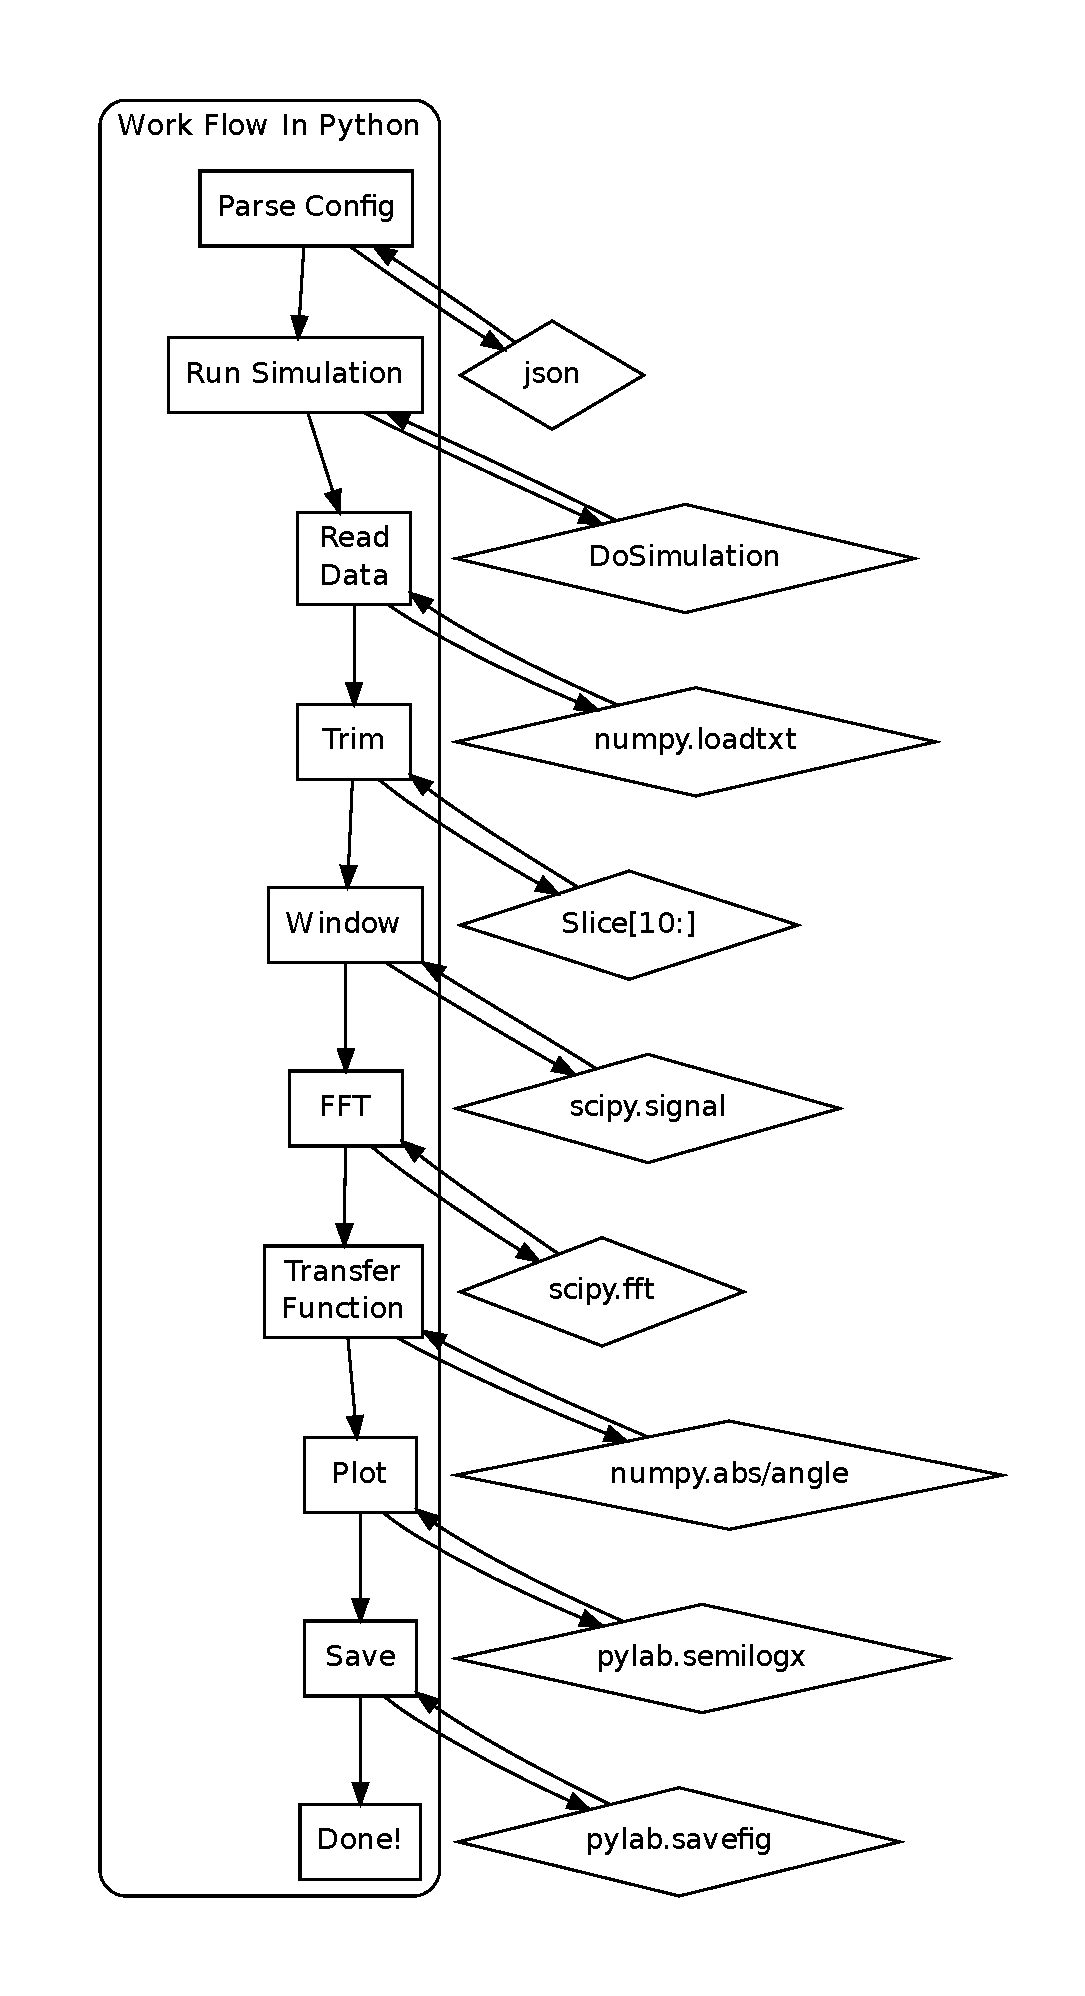
\includegraphics[height=0.85\textheight]{figures/TB_py_flow}
    \end{column}
  \end{columns}
}


\subsection{Configuration files}
% \frame{
%   \frametitle[]{Configuration files}
%     Details on JSON. Say what it is and why it's useful to use for interaction with upper levels.
% }

\frame{
  \frametitle[]{Configuration files}
  \begin{columns}[t]
      \begin{column}{0.5\textwidth}
 
        JavaScript Object Notation (JSON)
	\begin{itemize}
	\item Widely used standard
	\item Easy for humans to read and write
	\item Easy for computers to parse and generate
	\item Libraries available in many languages
	\end{itemize}
    
 
      \end{column}
      \begin{column}{0.5\hsize}
     \fontsize{7pt}{0pt}\selectfont
    \verbatiminput{quotes/one_linac_pt1.cfg}
      \end{column}
   \end{columns}
}

\frame{
  \frametitle[]{Configuration files}
\begin{columns}[t]
      \begin{column}{0.5\textwidth}
		Simulation Specific Properties
	\begin{itemize}
	\item  "Object Oriented"
	\begin{itemize}
	\item Layers represent physical structures of the accelerator
	\item Parameters associated to an object grouped
	\item Likewise the layers attempt to mirror data structures in the code
	\end{itemize}
          \item Fundamental parameters only
        \item Symbolic expressions  evaluated
	\end{itemize}
      \end{column}
      \begin{column}{0.5\hsize}
     \fontsize{7pt}{0pt}\selectfont
    \verbatiminput{quotes/one_linac_pt2.cfg}
      \end{column}
   \end{columns}
}


\frame{
  \frametitle[]{Input Scripting}

  Dictionaries can be specified instead of filename for easy scripting of parameter searches.

  Can operate as a command line script:
  \verbatiminput{quotes/cli.txt}

  Or use the Python function to call: 
  \verbatiminput{quotes/pythonscript.txt}

}

\frame{
  \frametitle[]{Example Parameter Search}
  Python's multiprocessing library makes multi core batching easy.

  See multiprocessing.Pool.map().

  \centerline{
  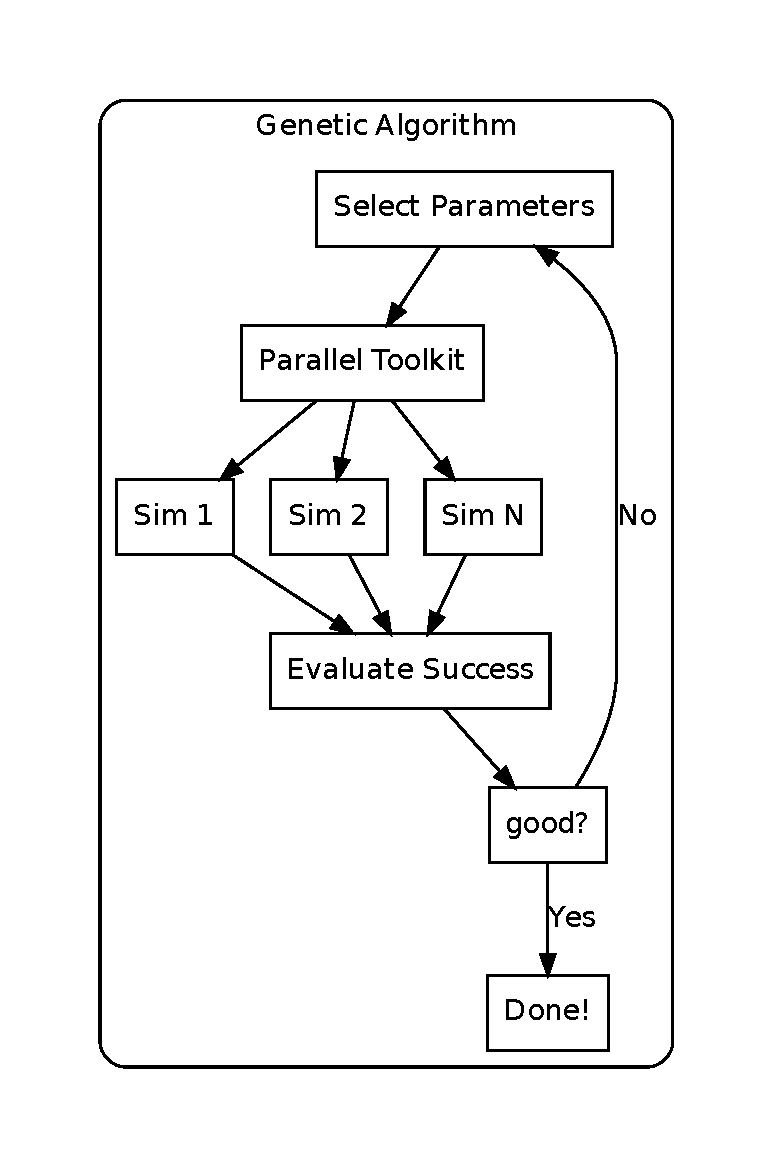
\includegraphics[height=0.8\textheight]{figures/gen_alg.pdf}
  }
}

\subsection{Front End}
\frame{
  \frametitle[]{Front End}
    \begin{itemize}
     \item ATG is migrating to JavaScript-based front ends,
     \item Server/client architecture where server generates JSON files and runs models,
     \item No need to install software or dependencies locally to run models and visualize results: Models can run in a powerful server to serve several clients,
     \item User-friendly interface enabling focus on science and hiding implementation details from the user.
    \end{itemize}

}

\section[Conclusions]{Conclusions and future improvements}
\frame{
	\frametitle[]{Conclusions and future improvements}
	\tableofcontents[currentsection, hideothersubsections]
}

\subsection{Conclusions}
\frame{
	\frametitle[]{Conclusions}
  \begin{itemize}
    \item Challenging project completed in a very small amount of time and surpassing expectations.
    \item Back-end simulation engine at a working stage: 
    \begin{itemize}
     \item Ready to produce Physics results without intricate knowledge of the implementation details,
     \item Easy to configure and to extend capabilities both in the back-end and the interfaces.
    \end{itemize}
    \item Strategic interest for involvement in projects related to LLRF and beam stability studies (not only NGLS).
    \item First ATG@LBNL project in a very exciting collaboration with UC Berkeley.
   \end{itemize}

}

\subsection{Future improvements}
\frame{
	\frametitle[]{Future improvements}
  \begin{itemize}
   \item Extension of models:
   \begin{itemize}
    \item Research on Beam-based feedback to find the optimal reading/actuator configuration and settings,
    \item Add more accurate models for beam instrumentation (currently characterized by estimated noise),
    \item Integrate micro-phonics (work done in Matlab by C. Rivetta),
    \item Include non-relativistic models or interface with existing ones,
    \item Add laser feedback system to refine gun noise characterization.
   \end{itemize}
  \item Possible re-implementation of the back-end in an FPGA (partially available).
  \end{itemize}

}

\frame{
	\frametitle[]{Questions?}
  \begin{figure}
    \centering
    
\includegraphics[scale=0.5]{figures/question_mark2.pdf}
  \end{figure}
}



\end{document} 
